\documentclass[11pt]{article}
\usepackage{amsmath, amssymb}
\usepackage[margin=1in]{geometry}
\usepackage{parskip}
\usepackage{graphicx}
\usepackage{booktabs}

\title{\textbf{Copper Reflectance Model\,---\,BBRsim Brief}}
\author{Golwala / Mirabolfathi group}
\date{}

\begin{document}
\maketitle

\tableofcontents
\bigskip

% ─────────────────────────────────────────────────────────────────────────────
\section{Conductivity}

The room-temperature conductivity of copper is universal across all grades:
\[
  \sigma_\mathrm{RT} = 5.96\times10^{7}\ \mathrm{S/m}
\]
At cryogenic temperature $T$ with residual resistance ratio $\mathrm{RRR}$,
Matthiessen's rule gives the total scattering rate as the sum of
impurity and phonon contributions:
\[
  \frac{1}{\sigma(T,\mathrm{RRR})}
  = \frac{1}{\sigma_\mathrm{impurity}} + \frac{1}{\sigma_\mathrm{phonon}(T)},
  \qquad
  \sigma_\mathrm{impurity} = \mathrm{RRR}\times\sigma_\mathrm{RT},
  \qquad
  \sigma_\mathrm{phonon}(T) \approx \sigma_\mathrm{RT}\,\frac{273\,\mathrm{K}}{T}.
\]
At $T = 4\,\mathrm{K}$ phonon scattering is frozen out and
$\sigma_\mathrm{DC}(4\,\mathrm{K}) \simeq \mathrm{RRR}\times\sigma_\mathrm{RT}$.
At $T = 273\,\mathrm{K}$ the result is $\sigma_\mathrm{RT}$ regardless of RRR,
consistent with the RRR definition.

\medskip
The \textbf{plasma frequency} of copper (free-electron model):
\[
  \omega_p = \sqrt{\frac{n_e e^2}{\varepsilon_0 m_e}}
  \approx 1.64\times10^{16}\ \mathrm{rad/s}
  \quad\Longrightarrow\quad
  f_p \approx 2.6\ \mathrm{PHz}\ \text{(UV)},
\]
where the material constants are listed in Section~\ref{sec:constants}.
We will see that $\omega_p$ sets the upper limit of metallic reflection.

% ─────────────────────────────────────────────────────────────────────────────
\section{Drude Scattering Time}

The electron scattering time $\tau$ connects the DC conductivity to the
free-electron Drude picture:
\[
  \tau = \frac{\sigma_\mathrm{DC}\, m_e}{n_e\, e^2}
       = \frac{\sigma_\mathrm{DC}}{\varepsilon_0\,\omega_p^2}.
\]
A useful identity: $\sigma_\mathrm{DC} = \varepsilon_0\,\omega_p^2\,\tau$.

\begin{center}
\begin{tabular}{@{}lll@{}}
\toprule
Symbol & Value & Meaning \\
\midrule
$n_e$ & $8.49\times10^{28}\ \mathrm{m}^{-3}$ & free electron density \\
$m_e$ & $9.109\times10^{-31}\ \mathrm{kg}$   & electron mass \\
$e$   & $1.602\times10^{-19}\ \mathrm{C}$    & electron charge \\
$\omega_p$ & $1.64\times10^{16}\ \mathrm{rad/s}$ & plasma angular frequency \\
\bottomrule
\end{tabular}
\end{center}

For OFHC Cu ($\mathrm{RRR}=100$) at $4\,\mathrm{K}$:
$\sigma_\mathrm{DC} = 5.96\times10^{9}\ \mathrm{S/m}$ and
$\tau \approx 2.5\ \mathrm{ps}$.

% ─────────────────────────────────────────────────────────────────────────────
\section{Drude AC Conductivity and Taylor Approximations}
\label{sec:ac}

The frequency-dependent (AC) conductivity from the Drude model:
\[
  \sigma(\omega)
  = \frac{\sigma_\mathrm{DC}}{1 - i\omega\tau}
  = \frac{\sigma_\mathrm{DC}(1+i\omega\tau)}{1+\omega^2\tau^2}.
\]
The real and imaginary parts are:
\[
  \mathrm{Re}[\sigma(\omega)] = \frac{\sigma_\mathrm{DC}}{1+(\omega\tau)^2},
  \qquad
  \mathrm{Im}[\sigma(\omega)] = \frac{\sigma_\mathrm{DC}\,\omega\tau}{1+(\omega\tau)^2}.
\]
$\mathrm{Im}[\sigma]$ peaks at $\omega\tau = 1$ with value $\sigma_\mathrm{DC}/2$.

\subsection*{Low-frequency limit ($\omega\tau \ll 1$): Taylor series}

Expanding $\sigma(\omega) = \sigma_\mathrm{DC}\sum_{n=0}^\infty(i\omega\tau)^n$:
\begin{align*}
  \mathrm{Re}[\sigma(\omega)] &= \sigma_\mathrm{DC}
    \bigl[1 - (\omega\tau)^2 + (\omega\tau)^4 - \cdots\bigr], \\
  \mathrm{Im}[\sigma(\omega)] &= \sigma_\mathrm{DC}
    \bigl[\omega\tau - (\omega\tau)^3 + \cdots\bigr].
\end{align*}
At leading order $\sigma(\omega)\to\sigma_\mathrm{DC}$: the DC conductivity
fully determines the optical response, giving the Hagen-Rubens limit.

\subsection*{High-frequency limit ($\omega\tau \gg 1$): Laurent series}

Writing $1/(1-i\omega\tau) = (i/\omega\tau)/(1+i/\omega\tau)$ and expanding:
\begin{align*}
  \mathrm{Re}[\sigma(\omega)] &= \frac{\sigma_\mathrm{DC}}{(\omega\tau)^2}
    \Bigl[1 - \frac{1}{(\omega\tau)^2} + \cdots\Bigr]
    \;\to\; \frac{\sigma_\mathrm{DC}}{(\omega\tau)^2}, \\[4pt]
  \mathrm{Im}[\sigma(\omega)] &= \frac{\sigma_\mathrm{DC}}{\omega\tau}
    \Bigl[1 - \frac{1}{(\omega\tau)^2} + \cdots\Bigr]
    \;\to\; \frac{\sigma_\mathrm{DC}}{\omega\tau}
           = \frac{n_e e^2}{m_e\,\omega}
           = \frac{\varepsilon_0\,\omega_p^2}{\omega}.
\end{align*}
In this regime the conductivity is almost purely imaginary (inductive).
The real part $\mathrm{Re}[\sigma]\propto(\omega\tau)^{-2}$ is the residual
dissipation.  The imaginary part at leading order $\varepsilon_0\omega_p^2/\omega$
is frequency-dependent and independent of $\tau$ — it encodes the inertia of
the electron gas, not its damping.

% ─────────────────────────────────────────────────────────────────────────────
\section{Complex Wave Vector (Griffiths \S9.4, complex $\sigma$)}

Griffiths \S9.4 derives, for a plane wave in a conductor,
$\tilde{k}^2 = \mu\varepsilon\omega^2 + i\mu\sigma\omega$.  With the
\emph{complex} Drude conductivity this becomes
\[
  \tilde{k}^2 = \frac{\omega^2}{c^2}\,\tilde{\varepsilon}(\omega),
  \qquad
  \tilde{\varepsilon}(\omega) = 1 + \frac{i\sigma(\omega)}{\varepsilon_0\omega}
  = 1 - \frac{\omega_p^2\tau^2}{1+\omega^2\tau^2}
      + \frac{i\,\omega_p^2\tau/\omega}{1+\omega^2\tau^2}.
\]
The negative real term — supplied by $\mathrm{Im}[\sigma]$ — is the
free-electron \emph{plasma} response.  It dominates
$\tilde{\varepsilon}$ throughout the BBRsim band and keeps the metal
highly reflective.  Griffiths's closed forms for $k$ and $\kappa$
(his eqs.\ 9.126) assume a \emph{real} $\sigma$ and must not be reused
with $\sigma_r = \mathrm{Re}[\sigma(\omega)]$ substituted in: doing so
drops the plasma term entirely.

The complex refractive index is $\tilde{n} = n + ik_\mathrm{opt} =
\sqrt{\tilde{\varepsilon}(\omega)}$.

\subsection*{Regime approximations}

Throughout the BBRsim range, $|\sigma(\omega)|/(\varepsilon_0\omega) \gg 1$
(\textbf{good-conductor limit}).  Writing
$\sigma(\omega) = |\sigma|e^{i\phi}$ with $\phi = \arctan(\omega\tau)$ and
$|\sigma| = \sigma_\mathrm{DC}/\sqrt{1+\omega^2\tau^2}$:
\[
  \tilde{n} \approx \sqrt{\frac{|\sigma|}{\varepsilon_0\omega}}\;
  e^{\,i\left(\frac{\pi}{4} + \frac{\phi}{2}\right)} .
\]

\smallskip
\noindent\textit{Low-$f$ ($\omega\tau\ll 1$, H-R regime):} $\phi\to 0$, so
\[
  n \approx k_\mathrm{opt} \approx
  \sqrt{\frac{\sigma_\mathrm{DC}}{2\varepsilon_0\omega}} \gg 1,
\]
the familiar skin-effect result with skin depth
$\delta = \sqrt{2/(\mu_0\sigma_\mathrm{DC}\omega)}$.

\smallskip
\noindent\textit{High-$f$ ($\omega\tau\gg 1$, relaxation regime):}
$\phi\to\pi/2$ and $|\sigma| \to \varepsilon_0\omega_p^2/\omega$, so
\[
  \tilde{n} \approx i\,\frac{\omega_p}{\omega}
  \qquad\Longrightarrow\qquad
  k_\mathrm{opt} \approx \frac{\omega_p}{\omega},
  \qquad
  n \approx \frac{\omega_p}{2\,\omega^2\tau} \ll k_\mathrm{opt}.
\]
$\tilde{n}$ is almost purely imaginary: the wave is screened by the inertia
of the electron gas rather than dissipated.  The field penetration depth
saturates at $c/\omega_p \approx 18$\,nm (the plasma penetration depth),
independent of frequency — the metal does \emph{not} become more
transparent above $f_\mathrm{break}$.

% ─────────────────────────────────────────────────────────────────────────────
\section{Reflectance and Absorptance}

Normal-incidence Fresnel reflectance from vacuum into the conductor:
\[
  \boxed{R = \left|\frac{\tilde{n}-1}{\tilde{n}+1}\right|^2
           = \frac{(n-1)^2 + k_\mathrm{opt}^2}{(n+1)^2 + k_\mathrm{opt}^2},}
  \qquad D = 1 - R.
\]
For $|\tilde{n}| \gg 1$ (good-conductor limit):
$D \approx 4n/|\tilde{n}|^2$.

\subsection*{Universal Drude formula}

With $\tilde{n} = \sqrt{|\sigma|/(\varepsilon_0\omega)}\,
e^{i(\pi/4+\phi/2)}$, $\phi = \arctan(\omega\tau)$:
\[
  \boxed{D(\omega)
  \approx D_\mathrm{HR}(\sigma_\mathrm{DC})\cdot
  \sqrt{2}\,\cos\!\left(\frac{\pi}{4}+\frac{\arctan\omega\tau}{2}\right)
  \left(1+\omega^2\tau^2\right)^{1/4},}
  \qquad
  D_\mathrm{HR} = 2\sqrt{\frac{2\varepsilon_0\omega}{\sigma_\mathrm{DC}}}.
\]
This single expression is valid throughout the BBRsim range.  It connects
the H-R limit continuously to the relaxation regime through the single
dimensionless parameter $\omega\tau$.

\subsection*{Limits of $D$}

\noindent\textit{Low-$f$ ($\omega\tau\ll 1$):}
\[
  D \to D_\mathrm{HR}, \qquad D \propto \omega^{1/2}.
\]

\noindent\textit{High-$f$ ($\omega\tau\gg 1$, $\omega\ll\omega_p$):}
the ratio falls as $1/\sqrt{2\omega\tau}$ and $D$ saturates at the
frequency-independent \emph{relaxation plateau}
\[
  \boxed{D \approx \frac{2}{\omega_p\tau}}
  \qquad\text{(OFHC Cu, RRR=100, 4\,K: } D \approx 4.9\times10^{-5}\text{).}
\]
Above $f_\mathrm{break}$ the absorptance rises \emph{more slowly} than the
H-R prediction (slope $\tfrac{1}{2}\to 0$): the plasma response screens the
field at the fixed depth $c/\omega_p$, while the per-cycle dissipation
$\mathrm{Re}[\sigma]\propto(\omega\tau)^{-2}$ falls exactly fast enough to
make $D$ flat.

\paragraph{Historical note (2026-06).}  Earlier revisions of this brief
substituted only $\sigma_r = \mathrm{Re}[\sigma(\omega)]$ into the real-$\sigma$
Griffiths formulas, which drops the plasma term and yields the erroneous
results $D/D_\mathrm{HR} = \sqrt{1+(\omega\tau)^2}$ and $D\propto\omega^{3/2}$
above $f_\mathrm{break}$ — overestimating absorption by ${\sim}30\times$ at
500\,GHz (RRR=100, 4\,K).  The full complex treatment above supersedes it.

% ─────────────────────────────────────────────────────────────────────────────
\section{Hagen-Rubens Limit and Breakdown Frequency}

In the limit $\omega\tau \ll 1$ (DC approximation), Eq.~(5) reduces to:
\[
  D = 1 - R \approx 2\sqrt{\frac{2\varepsilon_0\omega}{\sigma_\mathrm{DC}}}.
\]
This limit breaks down above the scattering frequency:
\[
  f_\mathrm{break} = \frac{1}{2\pi\tau}
  = \frac{n_e e^2}{2\pi\,m_e\,\sigma_\mathrm{DC}}.
\]

\begin{center}
\begin{tabular}{@{}lrrrr@{}}
\toprule
Grade & RRR & $\sigma_\mathrm{DC}$ [S/m] & $\tau$ [ps] & $f_\mathrm{break}$ [GHz] \\
\midrule
Commercial Cu    & 10  & $5.96\times10^{8}$ & 0.25 & 640 \\
OFHC Cu          & 100 & $5.96\times10^{9}$ & 2.5  & 64  \\
H$_2$-annealed   & 57  & $3.4\times10^{9}$  & 1.4  & 115 \\
Ultra-pure crystal & 500 & $3.0\times10^{10}$ & 12.5 & 13 \\
\bottomrule
\end{tabular}
\end{center}

BBRsim spans $50\ \mathrm{GHz}$--$20\ \mathrm{THz}$.
Hagen-Rubens is inadequate for essentially the entire range at cryogenic
temperatures: even for commercial Cu (RRR\,=\,10, $f_\mathrm{break}=640$\,GHz)
$\sim$97\% of the range lies above the limit.
\textbf{The full Drude model is always required.}

% ─────────────────────────────────────────────────────────────────────────────
\section{Regime Summary}

\begin{center}
\begin{tabular}{@{}llll@{}}
\toprule
Regime & Condition & $D \approx$ & log-log slope \\
\midrule
Hagen-Rubens (DC)   & $\omega\tau \ll 1$ &
  $2\sqrt{2\varepsilon_0\omega/\sigma_\mathrm{DC}}$ & $\tfrac{1}{2}$ \\[4pt]
Drude (full) & $\omega\tau \sim 1$ &
  $D_\mathrm{HR}\,\sqrt{2}\cos\!\bigl(\tfrac{\pi}{4}+\tfrac{\arctan\omega\tau}{2}\bigr)(1+\omega^2\tau^2)^{1/4}$ & $\tfrac{1}{2}\to 0$ \\[4pt]
Relaxation & $\omega\tau \gg 1$, $\omega\ll\omega_p$ &
  $2/(\omega_p\tau)$ \;(flat) & $0$ \\[4pt]
Plasma threshold & $\omega\to\omega_p$ &
  $R\to 0$ (transparent) & --- \\
\bottomrule
\end{tabular}
\end{center}

For copper, $f_p\approx 2.6$\,PHz (ultraviolet), so the plasma threshold is
far above the BBRsim range. The relevant transition in BBRsim is
H-R $\to$ relaxation, driven by $f_\mathrm{break}$.

\paragraph{Caveat — anomalous skin effect.}  At 4\,K and high RRR the electron
mean free path exceeds the classical penetration depth, and measured
cryogenic losses (Serov et al.\ 2016) sit above the classical relaxation
plateau.  The classical Drude model is the documented BBRsim baseline; an
ASE correction is a candidate refinement once O2 validation data exists.

% ─────────────────────────────────────────────────────────────────────────────
\section{Copper Material Constants}
\label{sec:constants}

\begin{center}
\begin{tabular}{@{}llll@{}}
\toprule
Constant & Symbol & Value & Units \\
\midrule
Room-temperature conductivity & $\sigma_\mathrm{RT}$ & $5.96\times10^{7}$ & S/m \\
Free electron density & $n_e$ & $8.49\times10^{28}$ & m$^{-3}$ \\
Electron mass & $m_e$ & $9.109\times10^{-31}$ & kg \\
Electron charge & $e$ & $1.602\times10^{-19}$ & C \\
Plasma frequency & $\omega_p$ & $1.64\times10^{16}$ & rad/s \\
Debye temperature & $\Theta_D$ & 343 & K \\
\bottomrule
\end{tabular}
\end{center}
$\sigma_\mathrm{RT}$ is universal for all copper grades.

% ─────────────────────────────────────────────────────────────────────────────
\section{Summary of Inputs}

All other quantities ($\sigma_\mathrm{DC}$, $\tau$, $\tilde{n}$, $R$) are
derived from just three inputs:

\begin{center}
\begin{tabular}{@{}ll@{}}
\toprule
Parameter & Meaning \\
\midrule
$\mathrm{RRR}$ & Residual resistance ratio; characterises Cu purity \\
$T\ [\mathrm{K}]$ & Temperature of the copper surface \\
$\omega = 2\pi f$ & Photon angular frequency \\
\bottomrule
\end{tabular}
\end{center}

% ─────────────────────────────────────────────────────────────────────────────
\section{Figures}

\begin{figure}[h!]
\centering
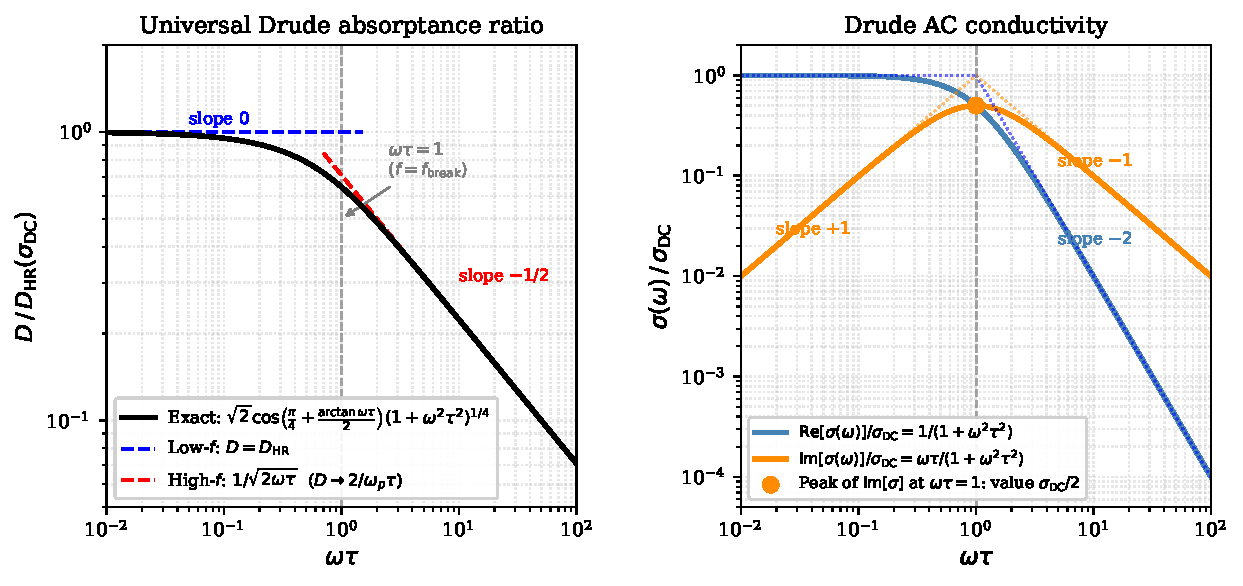
\includegraphics[width=\textwidth]{fig_drude_scaling.pdf}
\caption{%
  \textit{Left:} Universal Drude absorptance ratio $D/D_\mathrm{HR}$
  vs.\ dimensionless frequency $\omega\tau$.
  At $\omega\tau\ll 1$ (Hagen-Rubens regime), $D/D_\mathrm{HR}\to 1$.
  Above $\omega\tau=1$ ($f=f_\mathrm{break}$), the ratio falls as
  $1/\sqrt{2\omega\tau}$: $D$ saturates at the relaxation plateau
  $2/(\omega_p\tau)$ and the log-log slope of $D$ changes from
  $\tfrac{1}{2}$ to $0$.
  The exact closed form
  $\sqrt{2}\cos(\tfrac{\pi}{4}+\tfrac{\arctan\omega\tau}{2})(1+\omega^2\tau^2)^{1/4}$
  (solid line) and the two asymptotes (dashed) are shown.
  \textit{Right:} Real and imaginary parts of $\sigma(\omega)/\sigma_\mathrm{DC}$
  vs.\ $\omega\tau$.  Re$[\sigma]$ is a Lorentzian that rolls off as
  $(\omega\tau)^{-2}$; Im$[\sigma]$ peaks at $\omega\tau=1$ with value
  $\sigma_\mathrm{DC}/2$, then falls as $(\omega\tau)^{-1}$.
  Dotted lines indicate the asymptotic power laws.
}
\label{fig:drude_scaling}
\end{figure}

\begin{figure}[h!]
\centering
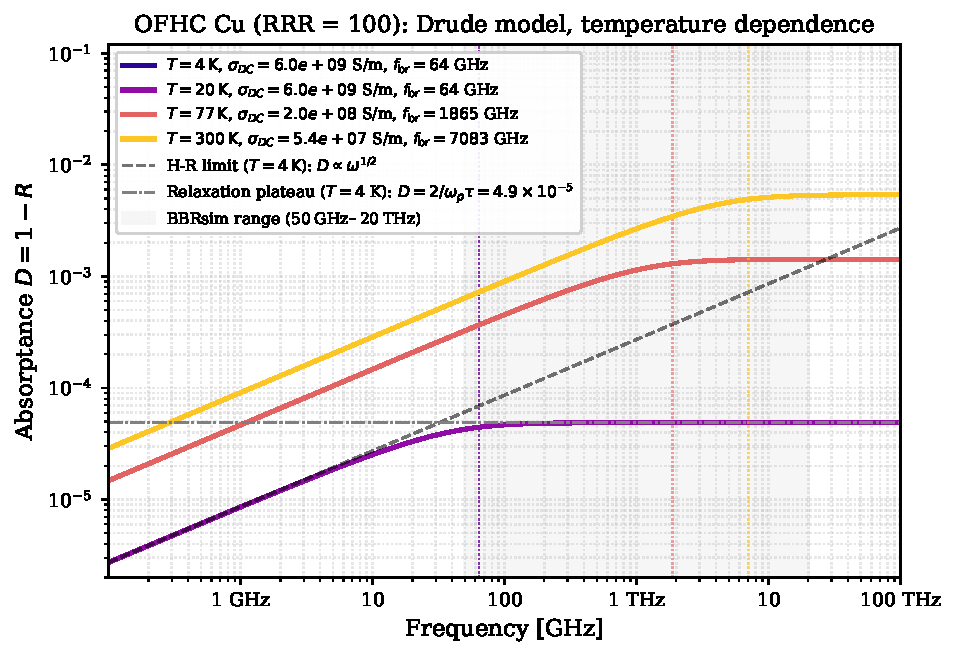
\includegraphics[width=0.82\textwidth]{fig_temp_dependence.pdf}
\caption{%
  Absorptance $D=1-R$ vs.\ frequency for OFHC Cu (RRR\,=\,100) at
  $T = 4, 20, 77, 300\,\mathrm{K}$ (full complex Drude model).
  Dotted vertical lines mark $f_\mathrm{break}=1/(2\pi\tau)$ for each
  temperature; above each line the curve flattens onto the relaxation
  plateau $D = 2/(\omega_p\tau)$ (grey dash-dot line for 4\,K).
  The dashed black line is the H-R approximation for $T=4\,\mathrm{K}$,
  which overestimates $D$ above $f_\mathrm{break}$.
  The gray band is the BBRsim simulation range (50\,GHz--20\,THz).
}
\label{fig:temp_dep}
\end{figure}

\end{document}
